The equation of circle can be expressed as
\begin{align}
    \vec{x}^T\vec{x}-2\vec{C}^T\vec{x}+f = 0
\end{align}
$\vec{C}$ is the centre  and substituting the points in the equation of circle we get
\begin{align}
2\myvec{1 & -2}\vec{C}-f &= 5\\
2\myvec{4 & -3}\vec{C}-f &= 25\\
\myvec{3 & 4}\vec{C} &= 7
\end{align}
can be expressed in matrix form
\begin{align}
\myvec{3 & 4 & 0 \\
2 & -4 & -1 \\
8 & -6 & -1}
\myvec{\vec{C}\\f} = \myvec{ 7 \\ 5 \\ 25}
\end{align}

Row reducing the augmented matrix
\begin{align}
\myvec{3 & 4 & 0 & 7\\
2 & -4 & -1 & 5 \\
8 & -6 & -1 & 25}
\xleftrightarrow{R_1\leftarrow R_1/3}
\myvec{1 & \frac{4}{3} & 0 & \frac{7}{3}\\ \\
2 & -4 & -1 & 5 \\ 
8 & -6 & -1 & 25}
\end{align}

\begin{align}
\xleftrightarrow[R_3\leftarrow R_3 - 8R_1]{R_2\leftarrow R_2 - 2R_1}
\myvec{1 & \frac{4}{3} & 0 & \frac{7}{3}\\ \\
0 & \frac{-20}{3} & -1 & \frac{1}{3} \\ \\
0 & \frac{-50}{3} & -1 & \frac{19}{3}}
\end{align}

\begin{align}
\xleftrightarrow{R_2\leftarrow \frac{-3}{20}R_2 }
\myvec{1 & \frac{4}{3} & 0 & \frac{7}{3}\\ \\
0 & 1 & \frac{3}{20} & \frac{-1}{20} \\ \\
0 & \frac{-50}{3} & -1 & \frac{19}{3}}
\end{align}

\begin{align}
\xleftrightarrow{R_3\leftarrow R_3 + \frac{50}{3}R_2}
\myvec{1 & \frac{4}{3} & 0 & \frac{7}{3}\\ \\
0 & 1 & \frac{3}{20} & \frac{-1}{20} \\ \\
0 & 0 & \frac{3}{2} & \frac{11}{2}}
\end{align}
\begin{align}
\vec{C} = \myvec{\frac{47}{15}  \\ \\ \frac{-3}{5} }
f = \frac{11}{3}
\end{align}
\begin{align}
f = \frac{11}{3}
\end{align}
The required circle equation,
\begin{align}
\vec{x}^T\vec{x}-2\myvec{\frac{47}{15} & \frac{-3}{5} }\vec{x} + \frac{11}{3} = 0
\end{align}

\begin{figure}[!ht]
\centering
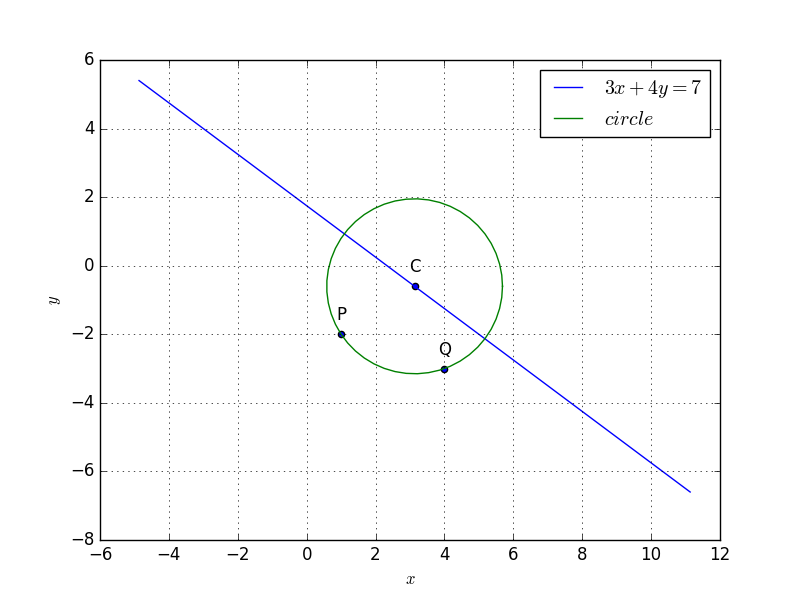
\includegraphics[width=\columnwidth]{./solutions/17/13/figure.png}
\caption{Circle passing through point P and Q also centre lie on the line 3x+4y=7}
\label{eq:solutions/17/13/Fig}
\end{figure}
